\section{Numerical framework}


%------------------------------------------------------------------------------

\begin{frame}
\frametitle{Compressible Navier Stokes equations}
The compressible Navier Stokes equations in conservative form can be written as
\begin{equation*}
\underbrace{\pdfrac{\av{\fstate}}{t}}_{\text{time derivative}} +
\underbrace{\nabla\cdot\fluxesconv(\av{\fstate})}_{\text{inviscid}} + 
\underbrace{\nabla\cdot\fluxesdiff(\av{\fstate})}_{\text{viscous}} =
\underbrace{\turbulencesource(\av{\fstate},\turbulenceparam_1,\cdots,\turbulenceparam_m)}_{\text{source term}}
\end{equation*}

Inviscid fluxes
\begin{align*}
\fluxesconv
%&=
%(\frac{1}{\dens} \fstate \T{\fstate} + \pres + \tensor{R}_3 \T{\fstate})
%\begin{bmatrix}
%\vec{0} \\ \eye_{3} \\ \vec{0}
%\end{bmatrix} \\ %TODO check if this one is correct
&=
\fstate \T{\fluidvel} + \pres
\begin{bmatrix}
0\\ \eye \\ \T{\fluidvel}
\end{bmatrix} \\
\end{align*}

Viscous fluxes
\begin{align*}\label{eq:fluxes_diff}
\fluxesdiff&=
\begin{bmatrix}
\vec{0}  \\
\fluidstress \\
\fluidstress \fluidvel + \heatflux
\end{bmatrix} \\
\end{align*}

\end{frame}

%------------------------------------------------------------------------------

\begin{frame}
\frametitle{Body-fitted vs. embedded framework}
\begin{columns}
\only<1->{\begin{column}{0.5\textwidth}
    Mesh is structure specific
    \begin{figure}
     \includegraphics[width=1.0\textwidth]{/home/lukas/Desktop/project/independence/project/thesis/fig/pdf/mesh_bodyfitted.pdf}
     \caption{Body-fitted}
     \end{figure}
\end{column}}
\only<2->{\begin{column}{0.5\textwidth}  %%<--- here
    Mesh independent of structure geometry
    \begin{figure}
     \includegraphics[width=1.0\textwidth]{/home/lukas/Desktop/project/independence/project/thesis/fig/pdf/mesh_embedded.pdf}
     \caption{Embedded}
     \end{figure}
\end{column}}
\end{columns}
\end{frame}


%------------------------------------------------------------------------------

%\begin{frame}
%\frametitle{Body-fitted vs. embedded framework}
%\begin{figure*}[b!]
%	\begin{subfigure}[t]{0.5\textwidth}
%	  \includegraphics[width=4cm]{/home/lukas/Desktop/project/independence/project/thesis/fig/pdf/mesh_bodyfitted.pdf}
%	  %\caption{aaa}
%	\end{subfigure}
%	\begin{subfigure}[t]{0.5\textwidth}
%	  \includegraphics[width=4cm]{/home/lukas/Desktop/project/independence/project/thesis/fig/pdf/mesh_embedded.pdf}
%	  %\caption{bbb}
%	\end{subfigure}
%  %\caption{ccc}
%\end{figure*}
%\end{frame}


%------------------------------------------------------------------------------

\begin{frame}
\frametitle{Immersed Boundary Method}
\framesubtitle{FIVER\footcite{Main2014}}
\begin{figure}[h!]
	\begin{center}
        \includegraphics[scale=0.75]{\thesispath/fig/tikz/build/fiver_surrogate_interface.pdf}
    \end{center}
\end{figure}
\end{frame}



%------------------------------------------------------------------------------

\begin{frame}
\frametitle{Discretization}
\begin{itemize}
 \item Body-fitted and Immersed boundaries (FIVER)
 \item FE-like treatment of the visocus term
\end{itemize}

\begin{align*}
\pdfrac{\fstate_i}{t} +
\int_{\partial\dualcell_i} \fluxesconv(\fstate)\cdot dS -
\int_{\sum_{T_i}} \difftensor \fstate \nabla \phi_i dx =
\vec{0}
\end{align*}


\begin{align*}
\int_{\partial\dualcell_i} \fluxesconv(\fstate)\cdot dS \approx
\underbrace{\sum_{j \in \vertexset(i)^a} \fluxesnum_{ij}(\fstate_{i},\fstate_{j},\wnormal_{ij})}_{\text{non-intersected elements}} +
\underbrace{\sum_{j \in \vertexset(i)\setminus\vertexset(i)^a} \fluxesnum_{ij}(\fstate_{i},\fstate^{*},\wnormal_{ij})}_{\text{intersected elements treated with FIVER}}
\end{align*}

$\fluxesnum$ ... flux function of Roe\footcite{Roe1981}

\end{frame}




%------------------------------------------------------------------------------

%\begin{frame}
%  \frametitle{CFD solver I: classical body fitted approach}
%  \vspace{-2mm}
%  \begin{block}{Body fitted CFD approach}
%    \begin{itemize}
%    \item Changes of the surface geometry require volume re-meshing or mesh deformation (ALE) \\[-1mm]
%    \item Re-meshing can be expensive and not fully automated  \\[-1mm]
%    \item Mesh deformation is not robust for large shape changes, 
%          cannot handle topological changes, and may be CPU intensive  \\[-1mm]
%    \item Convergence optimality requires computing the derivatives 
%          of the mesh changes in the entire computational fluid domain \\[-1mm]
%    \end{itemize}
%  \end{block}
%  \begin{figure}
%    \centering
%    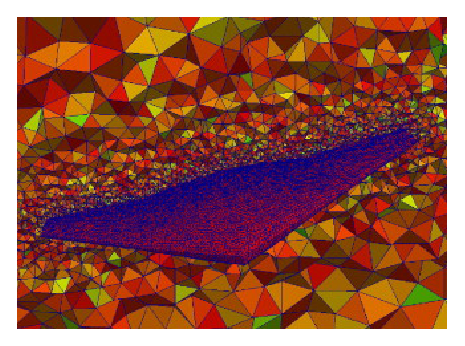
\includegraphics[width=0.44\textwidth]{Fig/mesh_def0}
%    \hspace{3mm}
%    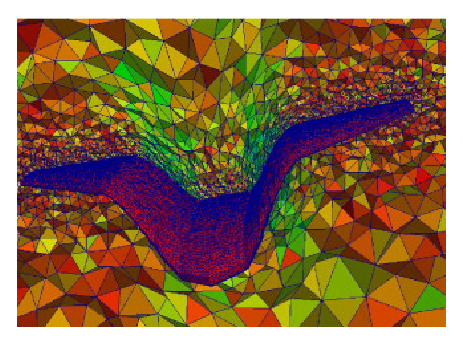
\includegraphics[width=0.44\textwidth]{Fig/mesh_def1}
%  \end{figure}
%\end{frame}

%------------------------------------------------------------------------------

%\begin{frame}
%  \frametitle{CFD solver II: non conforming grid approach}
%
%  \begin{block}{Immersed boundary CFD approach}
%    \begin{itemize}
%    \item Volume mesh does not conform to the surface mesh
%    \item Fixed volume mesh and decoupled geometry surface deformation 
%    \item Fast and robust mesh generation for geometry of arbitrary complexity
%    \item High level of automatization and flexible geometry modeling
%    \item Coupling between volume and surface discretization 
%      \begin{itemize}
%      \item Geometry intersector: can be fast, robust and accurate (CS)
%      \item IB numerical treatment: can be slow, not robust and not accurate (CFD)
%      \end{itemize}
%    \end{itemize}
%  \end{block}
%  \begin{figure}
%    \centering
%    \includegraphics[width=0.65\textwidth]{Fig/embopt}
%  \end{figure}
%
%\end{frame}

%------------------------------------------------------------------------------

%------------------------------------------------------------------------------

\begin{frame}
  \frametitle{IB with the FIVER approach: original formulation}
  \vspace{-2mm}
  \begin{itemize}
  \item Identify immersed boundaries with control volume interfaces $\mathcal{C}_{ij}$
    \begin{figure}[t!]
      \centering
      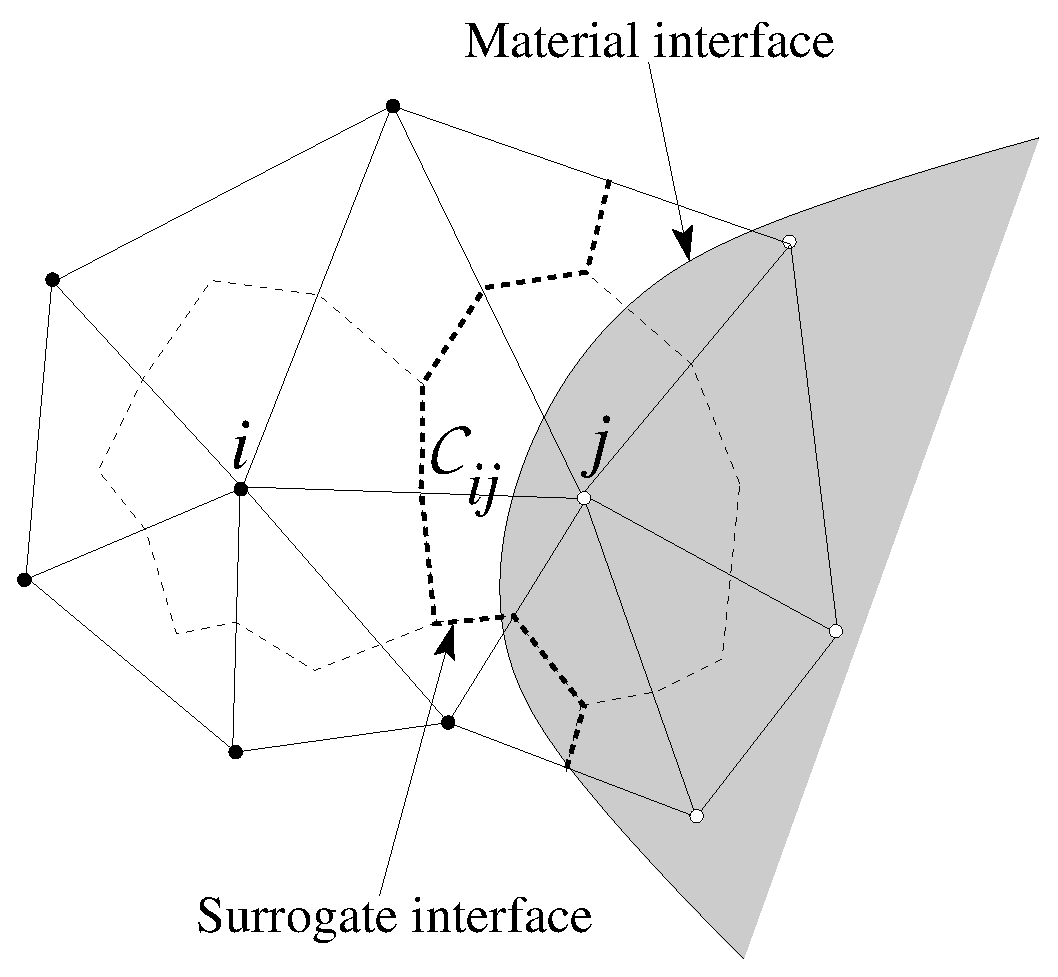
\includegraphics[width=0.35\textwidth]{Fig/fiver1}
    \end{figure} 
    \vspace{-1mm}
  \item Solve exactly local one-dimensional half-Riemann problems at $\mathcal{C}_{ij}$
    \vspace{-2mm}
    \begin{columns}
      \hspace{4mm}
      \begin{column}{0.55\textwidth}
        \begin{equation*}
          \left\{\!\!\!\! \begin{array}{ll}
            \dfrac{\partial \tilde\wbold^\star}{\partial \tau} + \dfrac{\partial\tilde\fbold(\tilde\wbold^\star)}{\partial \xi} = 0 \\[2mm]
            \tilde\wbold^\star(\xi, 0) = \tilde\wbold_{ij}, & \!\!\xi \le 0  \\[2mm]
            \vel(0, \tau)\cdot \nbold_\wall = \vel_\wall\cdot \nbold_\wall, & \!\!0 \le \tau \le \Delta t
          \end{array} \right.
        \end{equation*}
      \end{column}
      \begin{column}{0.43\textwidth}
        \begin{figure}[b!]
          \centering
          \hspace{-5mm}
          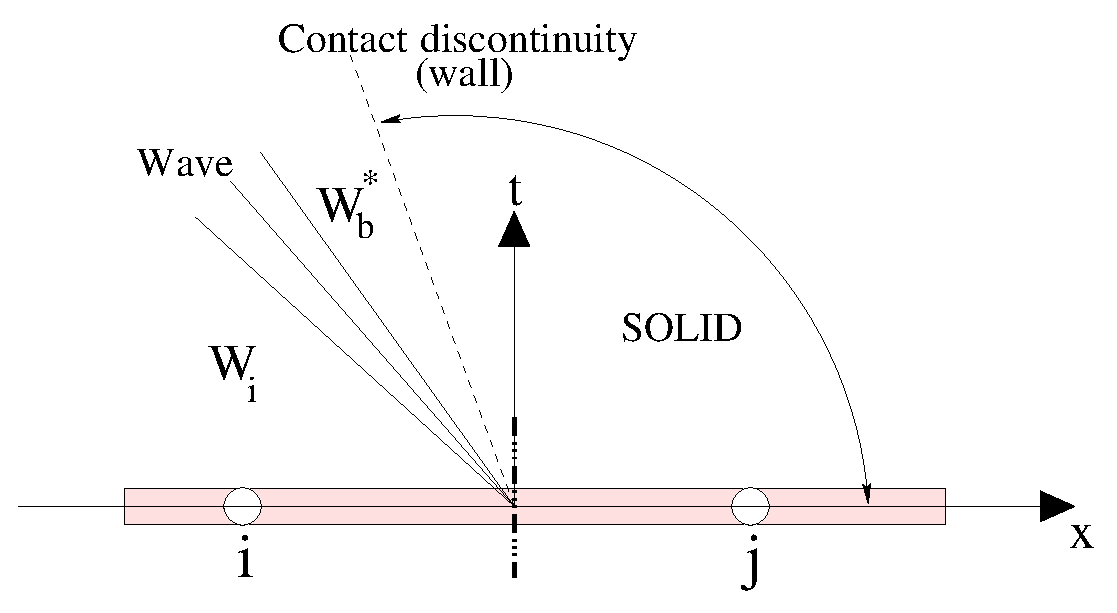
\includegraphics[width=0.99\textwidth]{Fig/riemann}
        \end{figure}
      \end{column}
    \end{columns}
    \item Evaluate numerical flux: $\Fbold_{ij} = \Fbold_{ij}(\wbold_{ij}, \wbold^\star_{b}, \n_{ij})$
  \end{itemize}
\end{frame}

%------------------------------------------------------------------------------

\begin{frame}
  \frametitle{IB with the FIVER approach: enhanced formulation}
  \begin{figure}[h!]
    \centering
    \includegraphics[width=0.35\textwidth]{Fig/fiver2}
  \end{figure}
  \vspace{-5mm}
  \begin{itemize}
  \item The fluid state is extrapolated to the material interface $\Gamma$ \\[-4mm]
    \begin{equation*}
      \wbold_\Gamma = \wbold_i + \nabla \wbold_i \boldsymbol\!\cdot (\xbold_\Gamma - \xbold_i)
    \end{equation*} 
  \item The one-dimensional half-Riemann problem is solved at material interface $\Gamma$\\[-4mm]
    \begin{equation*}
      \tilde\wbold^\star_\Gamma =\tilde\wbold^\star(\tilde\wbold_\Gamma, \vel_\wall, \nbold_\wall)
    \end{equation*} 
  \item The fluid state is inter/extra-polated at control volume interface $\mathcal{C}_{ij}$\\[-4mm]
    \begin{equation*}
      \wbold^\star_{ij} = \wbold^\star_{ij}(\wbold^\star_\Gamma, \wbold_{i'})
    \end{equation*}
  \item Numerical flux at the control volume interface: $\Fbold_{ij} = \Fbold_{ij}(\wbold_{ij}, \wbold^\star_{ij}, \n_{ij})$
  \item  Second-order convergence is recovered in the vicinity of the interface
  \end{itemize}
\end{frame}


%------------------------------------------------------------------------------


